\documentclass[a4paper,10pt]{article}

\usepackage[T1]{fontenc}
\usepackage[utf8]{inputenc}
\usepackage{mathtools}
\usepackage{graphicx}
\usepackage[margin=1in]{geometry}
\usepackage[spanish,activeacute]{babel}
\usepackage{hyperref}
\usepackage{fancyhdr}
\usepackage{incgraph,tikz}
\pagestyle{fancy}

\usepackage{color}
\usepackage{listings}
\lstset{ %
basicstyle=\footnotesize,       % the size of the fonts that are used for the code
numbers=left,                   % where to put the line-numbers
numberstyle=\footnotesize,      % the size of the fonts that are used for the line-numbers
stepnumber=1,                   % the step between two line-numbers. If it is 1 each line will be numbered
numbersep=10pt,                  % how far the line-numbers are from the code
backgroundcolor=\color{white},  % choose the background color. You must add \usepackage{color}
showspaces=false,               % show spaces adding particular underscores
showstringspaces=false,         % underline spaces within strings
showtabs=false,                 % show tabs within strings adding particular underscores
frame=single,           % adds a frame around the code
tabsize=4,          % sets default tabsize to 2 spaces
captionpos=b,           % sets the caption-position to bottom
breaklines=true,        % sets automatic line breaking
breakatwhitespace=false,    % sets if automatic breaks should only happen at whitespace
escapeinside={\%*}{*)}          % if you want to add a comment within your code
}
\renewcommand{\lstlistingname}{Código}
\usepackage{float}
\restylefloat{table}
\makeatletter
\def\verbatim{\small\@verbatim \frenchspacing\@vobeyspaces \@xverbatim}
\makeatother

\title{Speaker Recognition}

\lhead{Métodos Numéricos Avanzados}
\rhead{Análisis Armónico: Speaker Recognition}

\begin{document}

\begin{center}
\textbf{\Huge{Speaker Recognition}}
\end{center}

\begin{center}
\textbf{INTEGRANTES: Meola Franco Román, Puente Julieta, Strubolini Diego Martín}

\textbf{ITBA Segundo Cuatrimestre 2014}
\end{center}

\begin{center}
\text{PALABRAS CLAVE: análisis armónico, speaker recognition, mfcc, transformada de fourier, mel-frecuencia, mel-cepstral }
\end{center}

\begin{center}
\begin{large}
Resumen
\end{large}
\end{center}

Lorem ipsum dolor sit amet, consectetur adipiscing elit. Nullam id dolor id nibh ultricies vehicula ut id elit. Fusce dapibus, tellus ac cursus commodo, tortor mauris condimentum nibh, ut fermentum massa justo sit amet risus. Curabitur blandit tempus porttitor. Maecenas faucibus mollis interdum. Cum sociis natoque penatibus et magnis dis parturient montes, nascetur ridiculus mus. Lorem ipsum dolor sit amet, consectetur adipiscing elit.

\section{Introducción}
Lorem ipsum dolor sit amet, consectetur adipiscing elit. Nullam id dolor id nibh ultricies vehicula ut id elit. Fusce dapibus, tellus ac cursus commodo, tortor mauris condimentum nibh, ut fermentum massa justo sit amet risus. Curabitur blandit tempus porttitor. Maecenas faucibus mollis interdum. Cum sociis natoque penatibus et magnis dis parturient montes, nascetur ridiculus mus. Lorem ipsum dolor sit amet, consectetur adipiscing elit.

\section{Metodología}
Lorem ipsum dolor sit amet, consectetur adipiscing elit. Nullam id dolor id nibh ultricies vehicula ut id elit. Fusce dapibus, tellus ac cursus commodo, tortor mauris condimentum nibh, ut fermentum massa justo sit amet risus. Curabitur blandit tempus porttitor. Maecenas faucibus mollis interdum. Cum sociis natoque penatibus et magnis dis parturient montes, nascetur ridiculus mus. Lorem ipsum dolor sit amet, consectetur adipiscing elit.

\subsection{Implementación}
Lorem ipsum dolor sit amet, consectetur adipiscing elit. Nullam id dolor id nibh ultricies vehicula ut id elit. Fusce dapibus, tellus ac cursus commodo, tortor mauris condimentum nibh, ut fermentum massa justo sit amet risus. Curabitur blandit tempus porttitor. Maecenas faucibus mollis interdum. Cum sociis natoque penatibus et magnis dis parturient montes, nascetur ridiculus mus. Lorem ipsum dolor sit amet, consectetur adipiscing elit.
\newline

\begin{figure}[h]
\centering
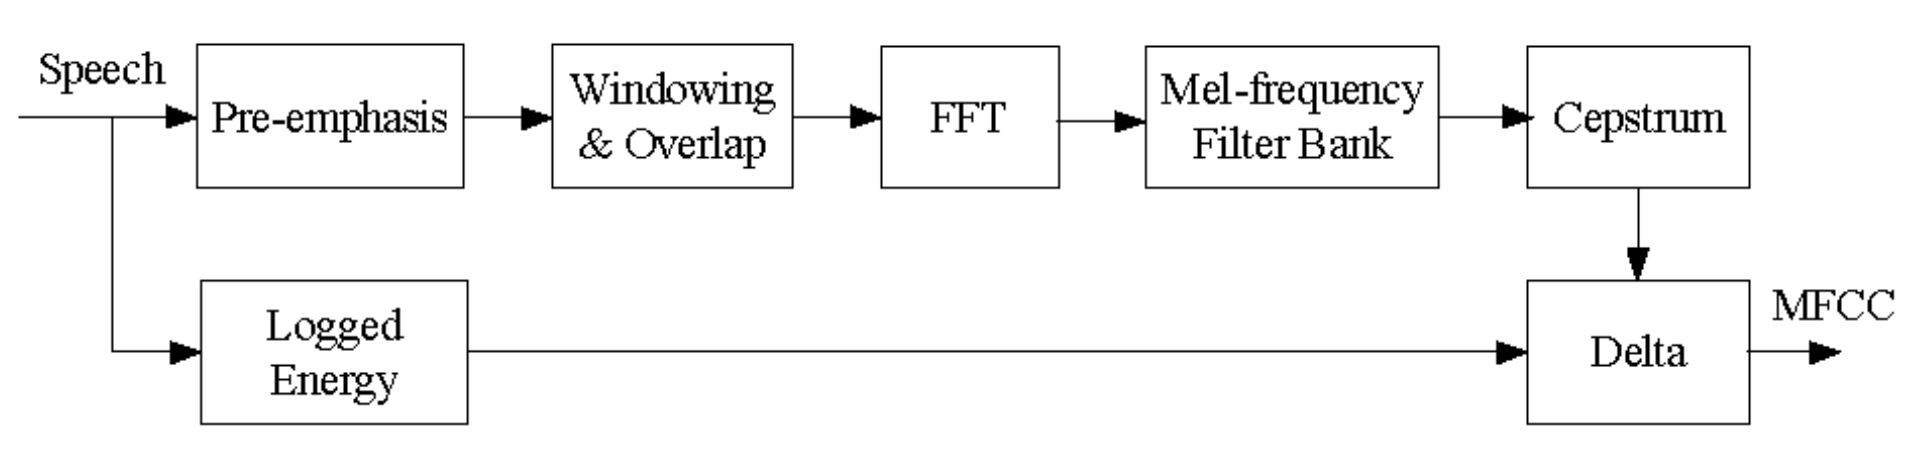
\includegraphics[width=\textwidth]{diagram}
\caption{Diagrama de Trabajo}
\end{figure}

Lorem ipsum dolor sit amet, consectetur adipiscing elit. Nullam id dolor id nibh ultricies vehicula ut id elit. Fusce dapibus, tellus ac cursus commodo, tortor mauris condimentum nibh, ut fermentum massa justo sit amet risus. Curabitur blandit tempus porttitor. Maecenas faucibus mollis interdum. Cum sociis natoque penatibus et magnis dis parturient montes, nascetur ridiculus mus. Lorem ipsum dolor sit amet, consectetur adipiscing elit.

\subsection{Función Principal}

\begin{lstlisting}[language=Octave, caption = mfcc.m]
\%*Llama a las demas funciones*)

function mfcc = mfcc(y,fv,fbanks)

overlap_percentage = 0.5;
frame = 0.02; \%20 ms

total_samples = rows(y);
frame_size = fv*frame;
overlap = overlap_percentage*frame_size;

yp = preemphasis(y,rows(y));

\%*figure(1);*)
\%*plot(y);*)
\%*title("$original$");*)

\%*figure(2);*)
\%*plot(yp);*)
\%*title("$preemphasis$");*)

\%*funcion de hamming*)
ham = hamming(frame_size);

total_frames = floor(total_samples/overlap)-1;

\%*Se iteran por los frames*)
\%*sacarle magic numbers*)
coef_amount = 13;
filter_amount = 33;

for f = 1: total_frames
    yw = windowing(yp,frame_size,f,overlap,ham);
    yf = fft(yw);
    yper = periodogram(yf,frame_size);
    \%*if f == 4*)
    \%*  figure(3)*)
    \%*  plot(yper);*)
    \%*end*)
    for fb = 1 : rows(fbanks)
    	energy = 0;
    	filterbank = fbanks(fb,:);
    	for fftpoint = 1 : columns(filterbank)
    		energy += filterbank(fftpoint)*yper(fftpoint);
    	end
    	filterenergies(fb)=energy;
    end
    for n = 1 : (coef_amount - 1)
    	c=0;
    	for k = 1 : filter_amount
    		c+=log(filterenergies(k))*cos(n*(k-0.5)*pi/filter_amount);
    	end
    	coef(n)=c;
    end
    energycoef = loggedenergy(y,frame_size);
    n+=1;
    coef(n)=energycoef;
    for k = 1 : n
        mfcc(k,f) = coef(k);
    end
end
\%*Se calculan los deltas*)
delta(1,:) = (2*(mfcc(:,3)) + (mfcc(:,2)))/10;
delta(2,:) = (2*(mfcc(:,4)) + (mfcc(:,3) - mfcc(:,1)))/10;
for f = 3 : (total_frames-2)
    delta(f,:) = (2*(mfcc(:,f+2) - mfcc(:,f-2)) + (mfcc(:,f+1) - mfcc(:,f-1)))/10;
end
delta(total_frames-1,:) = (2*(-1*mfcc(:,total_frames-3)) + (mfcc(:,total_frames) - mfcc(:,total_frames-2)))/10;
delta(total_frames,:) = (2*(-1*mfcc(:,total_frames-2)) + (-1*mfcc(:,total_frames-1)))/10;

\%*guardo los deltas*)
for f = 1 : total_frames
    for k = 1 : coef_amount
        mfcc(coef_amount + k,f) = delta(f,k);
    end
end

mfcc;
\end{lstlisting}


\begin{lstlisting}[language=Octave, caption = main.m]
function res = main()
sample_frequency = 8000;
filter_amount = 33;

fbanks = filterbanks(300,sample_frequency/2, filter_amount, 256);
[y,fv,bps] = wavread('media/JuanDaniela.wav');
coeforiginal = mfcc(y,fv,fbanks);
coefvqoriginal = vq(coeforiginal,16);

(...)

disp("Daniela");

[y,fv,bps] = wavread('media/HolaFranco.wav');
coefprueba1 = mfcc(y,fv,fbanks);
md1 = meandist(coefprueba1,coefvqoriginal);
disp(md1);

[y,fv,bps] = wavread('media/HolaSandra.wav');
coefprueba2 = mfcc(y,fv,fbanks);
md2 = meandist(coefprueba2,coefvqoriginal);
disp(md2);

(...)
\end{lstlisting}

\subsubsection{Pre-emphasis}

\begin{lstlisting}[language=Octave, caption = Pre-emphasis]
function yp = preemphasis(y, rows)

a = 0.97;
yp(1) = y(1);

for n = 2:rows
	yp(n) = y(n) - a * y(n-1);
end

yp;
\end{lstlisting}

\subsubsection{Windowing and Overlap}

\begin{lstlisting}[language=Octave, caption = Windowing]
function yw = windowing(y,frameSize,frameNmb,overlap, hamming)

i=1;
for k=1 + overlap*(frameNmb -1) : frameSize + overlap*(frameNmb-1)
	yw(i)=y(k)*hamming(i);
	i=i+1;
end

yw;
\end{lstlisting}

\subsubsection{FFT}

	Para el cálculo de la transformada de Fourier utilizamos el método \texttt{fft} provisto por Octave.

\subsubsection{Mel-frequency Filter Bank}

\begin{lstlisting}[language=Octave, caption = filterbanks]
function fb = filterbanks(min,max,amount,fftsize)

mmax = mel(max);
mmin = mel(min);
step = (mmax-mmin)/(amount+1);

for k=1:amount+2
	num = (k-1)*step + mmin;
	f(k) = num;
	fm(k) = melinv(num);
	fb(k) = floor((fftsize+1)*fm(k)/(max*2));
end

fbank = zeros(amount,fftsize/2+1);

for j=1:amount
	for i=fb(j):fb(j+1)
		fbank(j,i) = (i - fb(j))/(fb(j+1)-fb(j));
	end
	for i=fb(j+1):fb(j+2)
		fbank(j,i) = (fb(j+2)-i)/(fb(j+2)-fb(j+1));
	end
end

fb = fbank;
fb;
\end{lstlisting}

\subsubsection{Cepstrum}


\subsubsection{Logged Energy}

\begin{lstlisting}[language=Octave, caption = Logged Energy]
function energy = loggedenergy(y,framesize)

energy = 0;
for n = 1 : framesize
	energy += y(n)**2;
end;

energy = log(energy);	
energy;
\end{lstlisting}

\section{Resultados}
Lorem ipsum dolor sit amet, consectetur adipiscing elit. Nullam id dolor id nibh ultricies vehicula ut id elit. Fusce dapibus, tellus ac cursus commodo, tortor mauris condimentum nibh, ut fermentum massa justo sit amet risus. Curabitur blandit tempus porttitor. Maecenas faucibus mollis interdum. Cum sociis natoque penatibus et magnis dis parturient montes, nascetur ridiculus mus. Lorem ipsum dolor sit amet, consectetur adipiscing elit.
\newline

\begin{center}
\begin{table}[h]
\centering
\begin{tabular}{ccc}
\hline
\textbf{Persona} & \textbf{Coincidencia} & \textbf{Falsa Concidencia} \\ \hline
Franco&No&Enzo\\
Sandra&Si&-\\
Enzo&Si&-\\     
Paula&Si&-\\     
Diego&Si&-\\ 
Monica&No&Julieta\\
Julieta&No&Sandra\\
Daniela&No&Juli\\
Agustina&No&Sandra\\
Patricio&No&?\\
Sebastián&Si&-\\
\end{tabular}
\caption[Texto del índice (opcional)]{Susana}
\end{table}
\end{center}

\begin{center}
\begin{table}[h]
\centering
\begin{tabular}{ccc}
\hline
\textbf{Persona} & \textbf{Coincidencia} & \textbf{Falsa Concidencia} \\ \hline
Franco&No&Sandra\\
Sandra&No&Enzo\\
Enzo&Si&-\\     
Paula&Si&-\\     
Diego&Si&-\\ 
Monica&No&Julieta\\
Julieta&Si&-\\
Daniela&Si&-\\
Agustina&No&Julieta\\
Patricio&No&Sebastián\\
Sebastián&Si&-\\
\end{tabular}
\caption[Texto del índice (opcional)]{Juan}
\end{table}
\end{center}

\section{Conclusiones}
Lorem ipsum dolor sit amet, consectetur adipiscing elit. Nullam id dolor id nibh ultricies vehicula ut id elit. Fusce dapibus, tellus ac cursus commodo, tortor mauris condimentum nibh, ut fermentum massa justo sit amet risus. Curabitur blandit tempus porttitor. Maecenas faucibus mollis interdum. Cum sociis natoque penatibus et magnis dis parturient montes, nascetur ridiculus mus. Lorem ipsum dolor sit amet, consectetur adipiscing elit.

\section{Bibliografía}
\begin{itemize}

\item Wei Han, Cheong-Fat Chan, Chiu-Sing Choy, and Kong-Pang Pun. An ef- ficient mfcc extraction method in speech recognition. In Proceedings IEEE International Symposium on Circuits and Systems, 2006. ISCAS 2006., pa- ges 4 pp.–, May 2006.
\item Md Rashidul Hasan, Mustafa Jamil, Md Golam Rabbani, and Md Saifur Rahman. Speaker identification using mel frequency cepstral coefficients. In 3rd International Conference on Electrical \& Computer Engineering ICECE, volume 2004, 2004.
\item Y. Linde, A Buzo, and R.M. Gray. An algorithm for vector quantizer design. IEEE Transactions on Communications, 28(1):84–95, Jan 1980.
\item James Lyons. Mel frequency cepstral coefficient (mfcc) tutorial. 
\url{http://practicalcryptography.com/miscellaneous/machine-learning/guide-mel-frequency-cepstral-coefficients-mfccs/}
\item Manual de Funciones de Octave \url{https://www.gnu.org/software/octave/doc/interpreter/}
\end{itemize} 

\section{Funciones Auxiliares}

\begin{lstlisting}[language=Octave, caption = Mel]
function m = mel(f)

m = 1125*log(1+f/700);

m;
\end{lstlisting}

\begin{lstlisting}[language=Octave, caption = Mel Inversa]
function m = melinv(f)

m = 700*(exp(f/1125)-1);

m;
\end{lstlisting}

\begin{lstlisting}[language=Octave, caption = Periodogram]
function yp = periodogram(y,frameSize)

for k=1 : frameSize
  yp(k)= (abs(y(k))**2)/frameSize;
end

yp;
\end{lstlisting}

\end{document}